\subsection{Implementacja i dobór parametrów regulatora DMC 2x2}
\label{lab:zad4}



\ifdefined\CompileFigures
%\begin{figure}[H] 
%    \centering
%    % This file was created by matlab2tikz.
%
\definecolor{mycolor1}{rgb}{0.00000,0.44700,0.74100}%
%
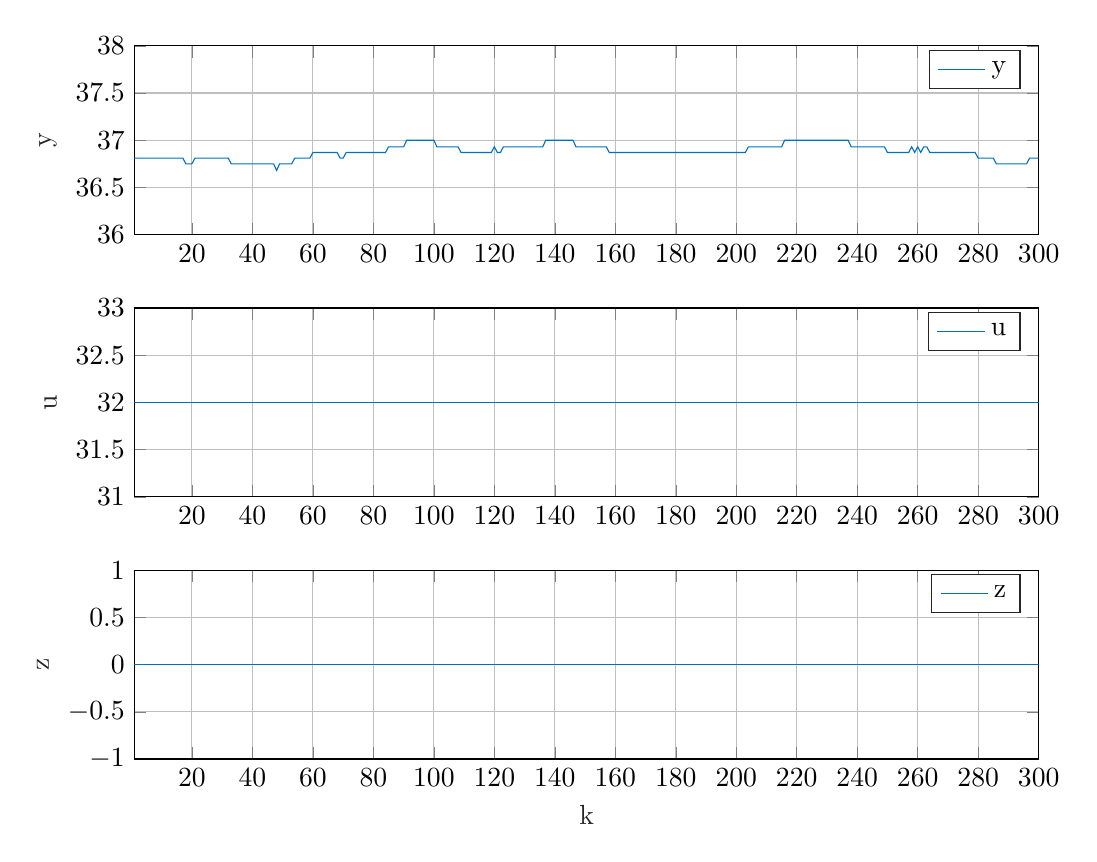
\begin{tikzpicture}

\begin{axis}[%
width=4.521in,
height=0.944in,
at={(0.758in,3.103in)},
scale only axis,
xmin=1,
xmax=300,
ymin=36,
ymax=38,
ylabel style={font=\color{white!15!black}},
ylabel={y},
axis background/.style={fill=white},
xmajorgrids,
ymajorgrids,
legend style={legend cell align=left, align=left, draw=white!15!black}
]
\addplot [color=mycolor1]
  table[row sep=crcr]{%
1	36.81\\
2	36.81\\
3	36.81\\
4	36.81\\
5	36.81\\
6	36.81\\
7	36.81\\
8	36.81\\
9	36.81\\
10	36.81\\
11	36.81\\
12	36.81\\
13	36.81\\
14	36.81\\
15	36.81\\
16	36.81\\
17	36.81\\
18	36.75\\
19	36.75\\
20	36.75\\
21	36.81\\
22	36.81\\
23	36.81\\
24	36.81\\
25	36.81\\
26	36.81\\
27	36.81\\
28	36.81\\
29	36.81\\
30	36.81\\
31	36.81\\
32	36.81\\
33	36.75\\
34	36.75\\
35	36.75\\
36	36.75\\
37	36.75\\
38	36.75\\
39	36.75\\
40	36.75\\
41	36.75\\
42	36.75\\
43	36.75\\
44	36.75\\
45	36.75\\
46	36.75\\
47	36.75\\
48	36.68\\
49	36.75\\
50	36.75\\
51	36.75\\
52	36.75\\
53	36.75\\
54	36.81\\
55	36.81\\
56	36.81\\
57	36.81\\
58	36.81\\
59	36.81\\
60	36.87\\
61	36.87\\
62	36.87\\
63	36.87\\
64	36.87\\
65	36.87\\
66	36.87\\
67	36.87\\
68	36.87\\
69	36.81\\
70	36.81\\
71	36.87\\
72	36.87\\
73	36.87\\
74	36.87\\
75	36.87\\
76	36.87\\
77	36.87\\
78	36.87\\
79	36.87\\
80	36.87\\
81	36.87\\
82	36.87\\
83	36.87\\
84	36.87\\
85	36.93\\
86	36.93\\
87	36.93\\
88	36.93\\
89	36.93\\
90	36.93\\
91	37\\
92	37\\
93	37\\
94	37\\
95	37\\
96	37\\
97	37\\
98	37\\
99	37\\
100	37\\
101	36.93\\
102	36.93\\
103	36.93\\
104	36.93\\
105	36.93\\
106	36.93\\
107	36.93\\
108	36.93\\
109	36.87\\
110	36.87\\
111	36.87\\
112	36.87\\
113	36.87\\
114	36.87\\
115	36.87\\
116	36.87\\
117	36.87\\
118	36.87\\
119	36.87\\
120	36.93\\
121	36.87\\
122	36.87\\
123	36.93\\
124	36.93\\
125	36.93\\
126	36.93\\
127	36.93\\
128	36.93\\
129	36.93\\
130	36.93\\
131	36.93\\
132	36.93\\
133	36.93\\
134	36.93\\
135	36.93\\
136	36.93\\
137	37\\
138	37\\
139	37\\
140	37\\
141	37\\
142	37\\
143	37\\
144	37\\
145	37\\
146	37\\
147	36.93\\
148	36.93\\
149	36.93\\
150	36.93\\
151	36.93\\
152	36.93\\
153	36.93\\
154	36.93\\
155	36.93\\
156	36.93\\
157	36.93\\
158	36.87\\
159	36.87\\
160	36.87\\
161	36.87\\
162	36.87\\
163	36.87\\
164	36.87\\
165	36.87\\
166	36.87\\
167	36.87\\
168	36.87\\
169	36.87\\
170	36.87\\
171	36.87\\
172	36.87\\
173	36.87\\
174	36.87\\
175	36.87\\
176	36.87\\
177	36.87\\
178	36.87\\
179	36.87\\
180	36.87\\
181	36.87\\
182	36.87\\
183	36.87\\
184	36.87\\
185	36.87\\
186	36.87\\
187	36.87\\
188	36.87\\
189	36.87\\
190	36.87\\
191	36.87\\
192	36.87\\
193	36.87\\
194	36.87\\
195	36.87\\
196	36.87\\
197	36.87\\
198	36.87\\
199	36.87\\
200	36.87\\
201	36.87\\
202	36.87\\
203	36.87\\
204	36.93\\
205	36.93\\
206	36.93\\
207	36.93\\
208	36.93\\
209	36.93\\
210	36.93\\
211	36.93\\
212	36.93\\
213	36.93\\
214	36.93\\
215	36.93\\
216	37\\
217	37\\
218	37\\
219	37\\
220	37\\
221	37\\
222	37\\
223	37\\
224	37\\
225	37\\
226	37\\
227	37\\
228	37\\
229	37\\
230	37\\
231	37\\
232	37\\
233	37\\
234	37\\
235	37\\
236	37\\
237	37\\
238	36.93\\
239	36.93\\
240	36.93\\
241	36.93\\
242	36.93\\
243	36.93\\
244	36.93\\
245	36.93\\
246	36.93\\
247	36.93\\
248	36.93\\
249	36.93\\
250	36.87\\
251	36.87\\
252	36.87\\
253	36.87\\
254	36.87\\
255	36.87\\
256	36.87\\
257	36.87\\
258	36.93\\
259	36.87\\
260	36.93\\
261	36.87\\
262	36.93\\
263	36.93\\
264	36.87\\
265	36.87\\
266	36.87\\
267	36.87\\
268	36.87\\
269	36.87\\
270	36.87\\
271	36.87\\
272	36.87\\
273	36.87\\
274	36.87\\
275	36.87\\
276	36.87\\
277	36.87\\
278	36.87\\
279	36.87\\
280	36.81\\
281	36.81\\
282	36.81\\
283	36.81\\
284	36.81\\
285	36.81\\
286	36.75\\
287	36.75\\
288	36.75\\
289	36.75\\
290	36.75\\
291	36.75\\
292	36.75\\
293	36.75\\
294	36.75\\
295	36.75\\
296	36.75\\
297	36.81\\
298	36.81\\
299	36.81\\
300	36.81\\
};
\addlegendentry{y}

\end{axis}

\begin{axis}[%
width=4.521in,
height=0.944in,
at={(0.758in,1.792in)},
scale only axis,
xmin=1,
xmax=300,
ymin=31,
ymax=33,
ylabel style={font=\color{white!15!black}},
ylabel={u},
axis background/.style={fill=white},
xmajorgrids,
ymajorgrids,
legend style={legend cell align=left, align=left, draw=white!15!black}
]
\addplot[const plot, color=mycolor1] table[row sep=crcr] {%
1	32\\
2	32\\
3	32\\
4	32\\
5	32\\
6	32\\
7	32\\
8	32\\
9	32\\
10	32\\
11	32\\
12	32\\
13	32\\
14	32\\
15	32\\
16	32\\
17	32\\
18	32\\
19	32\\
20	32\\
21	32\\
22	32\\
23	32\\
24	32\\
25	32\\
26	32\\
27	32\\
28	32\\
29	32\\
30	32\\
31	32\\
32	32\\
33	32\\
34	32\\
35	32\\
36	32\\
37	32\\
38	32\\
39	32\\
40	32\\
41	32\\
42	32\\
43	32\\
44	32\\
45	32\\
46	32\\
47	32\\
48	32\\
49	32\\
50	32\\
51	32\\
52	32\\
53	32\\
54	32\\
55	32\\
56	32\\
57	32\\
58	32\\
59	32\\
60	32\\
61	32\\
62	32\\
63	32\\
64	32\\
65	32\\
66	32\\
67	32\\
68	32\\
69	32\\
70	32\\
71	32\\
72	32\\
73	32\\
74	32\\
75	32\\
76	32\\
77	32\\
78	32\\
79	32\\
80	32\\
81	32\\
82	32\\
83	32\\
84	32\\
85	32\\
86	32\\
87	32\\
88	32\\
89	32\\
90	32\\
91	32\\
92	32\\
93	32\\
94	32\\
95	32\\
96	32\\
97	32\\
98	32\\
99	32\\
100	32\\
101	32\\
102	32\\
103	32\\
104	32\\
105	32\\
106	32\\
107	32\\
108	32\\
109	32\\
110	32\\
111	32\\
112	32\\
113	32\\
114	32\\
115	32\\
116	32\\
117	32\\
118	32\\
119	32\\
120	32\\
121	32\\
122	32\\
123	32\\
124	32\\
125	32\\
126	32\\
127	32\\
128	32\\
129	32\\
130	32\\
131	32\\
132	32\\
133	32\\
134	32\\
135	32\\
136	32\\
137	32\\
138	32\\
139	32\\
140	32\\
141	32\\
142	32\\
143	32\\
144	32\\
145	32\\
146	32\\
147	32\\
148	32\\
149	32\\
150	32\\
151	32\\
152	32\\
153	32\\
154	32\\
155	32\\
156	32\\
157	32\\
158	32\\
159	32\\
160	32\\
161	32\\
162	32\\
163	32\\
164	32\\
165	32\\
166	32\\
167	32\\
168	32\\
169	32\\
170	32\\
171	32\\
172	32\\
173	32\\
174	32\\
175	32\\
176	32\\
177	32\\
178	32\\
179	32\\
180	32\\
181	32\\
182	32\\
183	32\\
184	32\\
185	32\\
186	32\\
187	32\\
188	32\\
189	32\\
190	32\\
191	32\\
192	32\\
193	32\\
194	32\\
195	32\\
196	32\\
197	32\\
198	32\\
199	32\\
200	32\\
201	32\\
202	32\\
203	32\\
204	32\\
205	32\\
206	32\\
207	32\\
208	32\\
209	32\\
210	32\\
211	32\\
212	32\\
213	32\\
214	32\\
215	32\\
216	32\\
217	32\\
218	32\\
219	32\\
220	32\\
221	32\\
222	32\\
223	32\\
224	32\\
225	32\\
226	32\\
227	32\\
228	32\\
229	32\\
230	32\\
231	32\\
232	32\\
233	32\\
234	32\\
235	32\\
236	32\\
237	32\\
238	32\\
239	32\\
240	32\\
241	32\\
242	32\\
243	32\\
244	32\\
245	32\\
246	32\\
247	32\\
248	32\\
249	32\\
250	32\\
251	32\\
252	32\\
253	32\\
254	32\\
255	32\\
256	32\\
257	32\\
258	32\\
259	32\\
260	32\\
261	32\\
262	32\\
263	32\\
264	32\\
265	32\\
266	32\\
267	32\\
268	32\\
269	32\\
270	32\\
271	32\\
272	32\\
273	32\\
274	32\\
275	32\\
276	32\\
277	32\\
278	32\\
279	32\\
280	32\\
281	32\\
282	32\\
283	32\\
284	32\\
285	32\\
286	32\\
287	32\\
288	32\\
289	32\\
290	32\\
291	32\\
292	32\\
293	32\\
294	32\\
295	32\\
296	32\\
297	32\\
298	32\\
299	32\\
300	32\\
};
\addlegendentry{u}

\end{axis}

\begin{axis}[%
width=4.521in,
height=0.944in,
at={(0.758in,0.481in)},
scale only axis,
xmin=1,
xmax=300,
xlabel style={font=\color{white!15!black}},
xlabel={k},
ymin=-1,
ymax=1,
ylabel style={font=\color{white!15!black}},
ylabel={z},
axis background/.style={fill=white},
xmajorgrids,
ymajorgrids,
legend style={legend cell align=left, align=left, draw=white!15!black}
]
\addplot[const plot, color=mycolor1] table[row sep=crcr] {%
1	0\\
2	0\\
3	0\\
4	0\\
5	0\\
6	0\\
7	0\\
8	0\\
9	0\\
10	0\\
11	0\\
12	0\\
13	0\\
14	0\\
15	0\\
16	0\\
17	0\\
18	0\\
19	0\\
20	0\\
21	0\\
22	0\\
23	0\\
24	0\\
25	0\\
26	0\\
27	0\\
28	0\\
29	0\\
30	0\\
31	0\\
32	0\\
33	0\\
34	0\\
35	0\\
36	0\\
37	0\\
38	0\\
39	0\\
40	0\\
41	0\\
42	0\\
43	0\\
44	0\\
45	0\\
46	0\\
47	0\\
48	0\\
49	0\\
50	0\\
51	0\\
52	0\\
53	0\\
54	0\\
55	0\\
56	0\\
57	0\\
58	0\\
59	0\\
60	0\\
61	0\\
62	0\\
63	0\\
64	0\\
65	0\\
66	0\\
67	0\\
68	0\\
69	0\\
70	0\\
71	0\\
72	0\\
73	0\\
74	0\\
75	0\\
76	0\\
77	0\\
78	0\\
79	0\\
80	0\\
81	0\\
82	0\\
83	0\\
84	0\\
85	0\\
86	0\\
87	0\\
88	0\\
89	0\\
90	0\\
91	0\\
92	0\\
93	0\\
94	0\\
95	0\\
96	0\\
97	0\\
98	0\\
99	0\\
100	0\\
101	0\\
102	0\\
103	0\\
104	0\\
105	0\\
106	0\\
107	0\\
108	0\\
109	0\\
110	0\\
111	0\\
112	0\\
113	0\\
114	0\\
115	0\\
116	0\\
117	0\\
118	0\\
119	0\\
120	0\\
121	0\\
122	0\\
123	0\\
124	0\\
125	0\\
126	0\\
127	0\\
128	0\\
129	0\\
130	0\\
131	0\\
132	0\\
133	0\\
134	0\\
135	0\\
136	0\\
137	0\\
138	0\\
139	0\\
140	0\\
141	0\\
142	0\\
143	0\\
144	0\\
145	0\\
146	0\\
147	0\\
148	0\\
149	0\\
150	0\\
151	0\\
152	0\\
153	0\\
154	0\\
155	0\\
156	0\\
157	0\\
158	0\\
159	0\\
160	0\\
161	0\\
162	0\\
163	0\\
164	0\\
165	0\\
166	0\\
167	0\\
168	0\\
169	0\\
170	0\\
171	0\\
172	0\\
173	0\\
174	0\\
175	0\\
176	0\\
177	0\\
178	0\\
179	0\\
180	0\\
181	0\\
182	0\\
183	0\\
184	0\\
185	0\\
186	0\\
187	0\\
188	0\\
189	0\\
190	0\\
191	0\\
192	0\\
193	0\\
194	0\\
195	0\\
196	0\\
197	0\\
198	0\\
199	0\\
200	0\\
201	0\\
202	0\\
203	0\\
204	0\\
205	0\\
206	0\\
207	0\\
208	0\\
209	0\\
210	0\\
211	0\\
212	0\\
213	0\\
214	0\\
215	0\\
216	0\\
217	0\\
218	0\\
219	0\\
220	0\\
221	0\\
222	0\\
223	0\\
224	0\\
225	0\\
226	0\\
227	0\\
228	0\\
229	0\\
230	0\\
231	0\\
232	0\\
233	0\\
234	0\\
235	0\\
236	0\\
237	0\\
238	0\\
239	0\\
240	0\\
241	0\\
242	0\\
243	0\\
244	0\\
245	0\\
246	0\\
247	0\\
248	0\\
249	0\\
250	0\\
251	0\\
252	0\\
253	0\\
254	0\\
255	0\\
256	0\\
257	0\\
258	0\\
259	0\\
260	0\\
261	0\\
262	0\\
263	0\\
264	0\\
265	0\\
266	0\\
267	0\\
268	0\\
269	0\\
270	0\\
271	0\\
272	0\\
273	0\\
274	0\\
275	0\\
276	0\\
277	0\\
278	0\\
279	0\\
280	0\\
281	0\\
282	0\\
283	0\\
284	0\\
285	0\\
286	0\\
287	0\\
288	0\\
289	0\\
290	0\\
291	0\\
292	0\\
293	0\\
294	0\\
295	0\\
296	0\\
297	0\\
298	0\\
299	0\\
300	0\\
};
\addlegendentry{z}

\end{axis}
\end{tikzpicture}%
%    \caption{Punkt pracy obiektu}
%    \label{lab:zad1:figure}
%\end{figure}
\fi

Na	sterowniku	zaimplementowano	uwzględniając	ograniczenia	regulator	DMC	
2x2	w	wersji	oszczędnej	obliczeniowo(analitycznej). Pozyskano	odpowiedzi	
skokowe	obiektu.	Dobierając	parametry	regulatora	uwzględniono:
Liczbę	wykorzystanych	rejestrów	pamięci,	czas	obliczeń	pojedynczej	iteracji	
algorytmu	oraz	jakość	regulacji
Implementacja	
Wykresy

\subsubsection{Implementacja}

\lstset{style=custommatlab}
\ifdefined\CompileListings
    \lstinputlisting[
        firstline=6, 
        lastline=41, 
        caption="Skrypt generujący parametry regulatora DMC"]
        {../lab/DMC/DMC_script.m}
    %\newpage
\fi

\lstset{style=custommatlab}
\ifdefined\CompileListings
    \lstinputlisting[
        firstline=6, 
        lastline=24, 
        caption="Skrypt wyliczający parametry regulatora DMC"]
        {../lab/DMC/DMC_init.m}
    \newpage
\fi

\lstset{style=custommatlab}
\ifdefined\CompileListings
    \lstinputlisting[
        firstline=6, 
        lastline=49, 
        caption="Skrypt eksportujący parametry regulatora DMC do pliku"]
        {../lab/DMC/exporter.m}
    \newpage
\fi

\lstset{style=custommatlab}
\ifdefined\CompileListings
    \lstinputlisting[
        firstline=1, 
        lastline=51, 
        caption="Wygenerowany program ST inicjujący regulatory DMC"]
        {../lab/DMC/DMC_data.st}
    \newpage
\fi

\lstset{style=customc}
\ifdefined\CompileListings
    \lstinputlisting[
        firstline=1, 
        lastline=39, 
        caption="Program ST implementujący algorytm DMC toru G1-T1"]
        {../lab/src/DMC_R_FixedScan.st}
    \newpage
\fi

\lstset{style=customc}
\ifdefined\CompileListings
    \lstinputlisting[
        firstline=42, 
        lastline=80, 
        caption="Program ST implementujący algorytm DMC toru G2-T3"]
        {../lab/src/DMC_R_FixedScan.st}
    \newpage
\fi

\subsubsection{Wyznaczenie wektorów s regulatorów DMC}


\ifdefined\CompileFigures
\begin{figure}[H] 
    \centering
    % This file was created by matlab2tikz.
%
\definecolor{mycolor1}{rgb}{0.00000,0.44700,0.74100}%
%
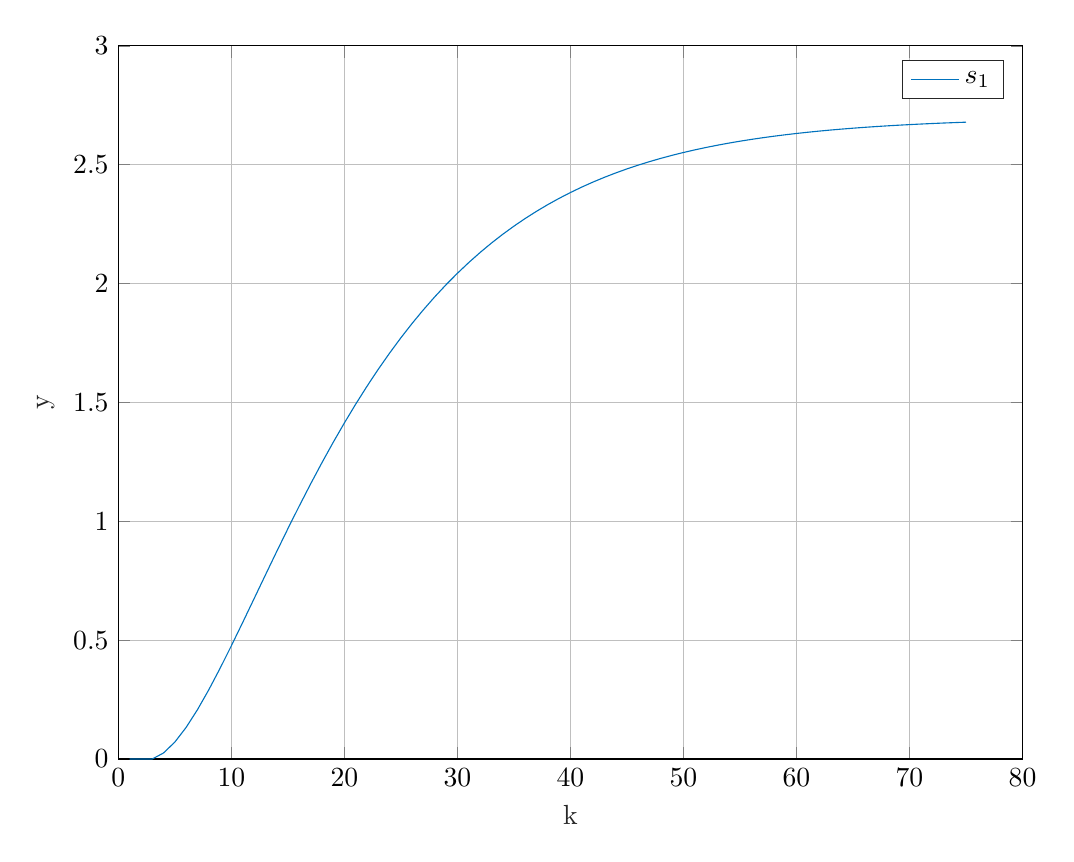
\begin{tikzpicture}

\begin{axis}[%
width=4.521in,
height=3.566in,
at={(0.758in,0.481in)},
scale only axis,
xmin=0,
xmax=80,
xlabel style={font=\color{white!15!black}},
xlabel={k},
ymin=0,
ymax=3,
ylabel style={font=\color{white!15!black}},
ylabel={y},
axis background/.style={fill=white},
xmajorgrids,
ymajorgrids,
legend style={legend cell align=left, align=left, draw=white!15!black}
]
\addplot [color=mycolor1]
  table[row sep=crcr]{%
1	0\\
2	0\\
3	0\\
4	0.0254293893029355\\
5	0.0712089201199524\\
6	0.133034368511904\\
7	0.20726956952784\\
8	0.290853518026229\\
9	0.381219733135963\\
10	0.476226311778269\\
11	0.574095295673299\\
12	0.673360150339118\\
13	0.772820306858862\\
14	0.871501850362001\\
15	0.968623555618423\\
16	1.06356757196428\\
17	1.15585414879211\\
18	1.24511987064386\\
19	1.33109893894391\\
20	1.41360709682677\\
21	1.49252784542365\\
22	1.56780064531436\\
23	1.639410836448\\
24	1.70738104440896\\
25	1.77176387108377\\
26	1.83263569412187\\
27	1.89009142256206\\
28	1.94424007603911\\
29	1.99520107246257\\
30	2.04310112429402\\
31	2.08807165682581\\
32	2.13024667342865\\
33	2.16976100280625\\
34	2.20674887206101\\
35	2.24134275700129\\
36	2.27367246775349\\
37	2.30386443350759\\
38	2.33204115523317\\
39	2.35832079955227\\
40	2.38281691072888\\
41	2.40563822100758\\
42	2.42688854236976\\
43	2.44666672523133\\
44	2.46506667173065\\
45	2.48217739309177\\
46	2.49808310213433\\
47	2.51286333336966\\
48	2.5265930843017\\
49	2.53934297256633\\
50	2.55117940441461\\
51	2.56216475079417\\
52	2.57235752792437\\
53	2.58181257980902\\
54	2.5905812605993\\
55	2.59871161511742\\
56	2.6062485561913\\
57	2.61323403773654\\
58	2.61970722276539\\
59	2.62570464570544\\
60	2.63126036858254\\
61	2.63640613076464\\
62	2.64117149208164\\
63	2.64558396923413\\
64	2.64966916548338\\
65	2.65345089368008\\
66	2.65695129274058\\
67	2.66019093772095\\
68	2.66318894367054\\
69	2.66596306347073\\
70	2.66852977988228\\
71	2.67090439203648\\
72	2.67310109661295\\
73	2.67513306395087\\
74	2.67701250934101\\
75	2.67875075974426\\
};
\addlegendentry{$\text{s}_\text{1}$}

\end{axis}
\end{tikzpicture}%
    \caption{Wektor s regulatora DMC  G1}
    \label{lab:zad4:figure:wektorS1}
 \end{figure}
\fi

\ifdefined\CompileFigures
\begin{figure}[H] 
    \centering
    % This file was created by matlab2tikz.
%
\definecolor{mycolor1}{rgb}{0.00000,0.44700,0.74100}%
%
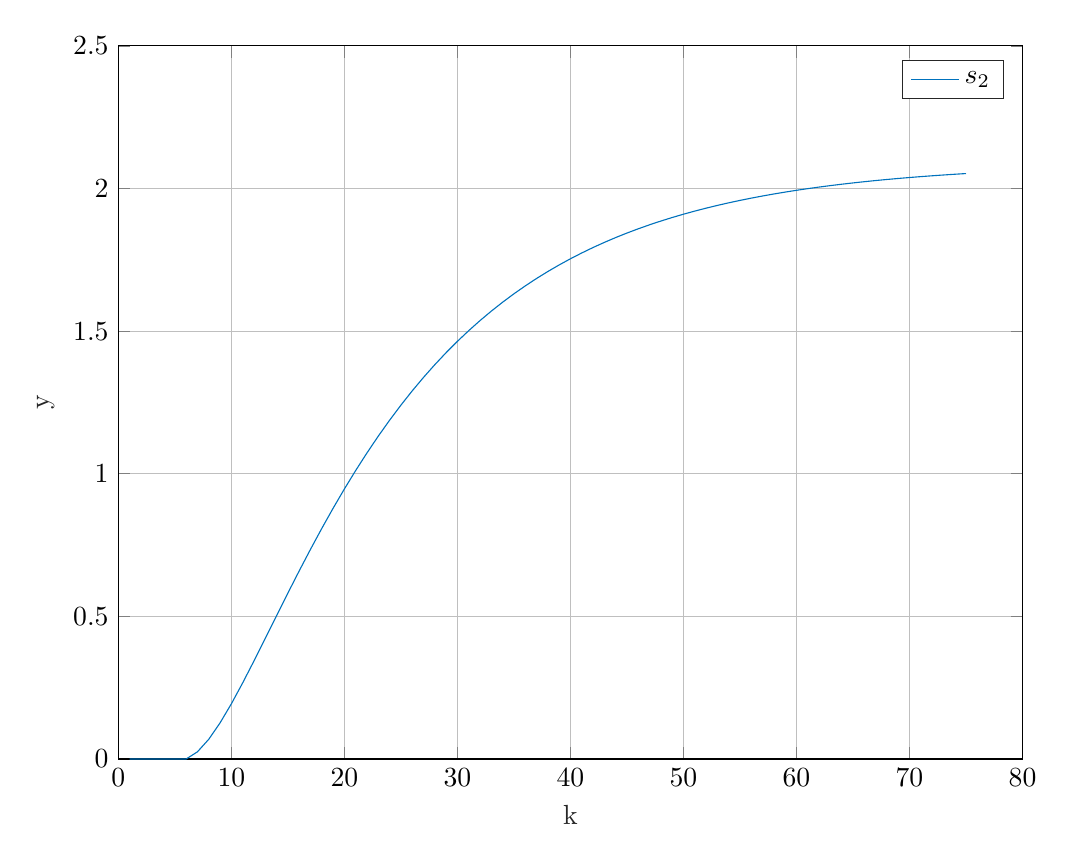
\begin{tikzpicture}

\begin{axis}[%
width=4.521in,
height=3.566in,
at={(0.758in,0.481in)},
scale only axis,
xmin=0,
xmax=80,
xlabel style={font=\color{white!15!black}},
xlabel={k},
ymin=0,
ymax=2.5,
ylabel style={font=\color{white!15!black}},
ylabel={y},
axis background/.style={fill=white},
xmajorgrids,
ymajorgrids,
legend style={legend cell align=left, align=left, draw=white!15!black}
]
\addplot [color=mycolor1]
  table[row sep=crcr]{%
1	0\\
2	0\\
3	0\\
4	0\\
5	0\\
6	0\\
7	0.0252319648469853\\
8	0.069139380226757\\
9	0.126564820810333\\
10	0.193465552531634\\
11	0.266686144684645\\
12	0.343776711316365\\
13	0.422847670352597\\
14	0.502453725659747\\
15	0.581501231927335\\
16	0.659174267007119\\
17	0.734875668941911\\
18	0.808180041623654\\
19	0.878796330880932\\
20	0.946538051473337\\
21	1.01129962871619\\
22	1.07303762529261\\
23	1.13175586946008\\
24	1.18749369751903\\
25	1.24031668084705\\
26	1.29030933383051\\
27	1.33756939990827\\
28	1.38220339369088\\
29	1.42432314174744\\
30	1.46404311637561\\
31	1.50147839806046\\
32	1.53674313544637\\
33	1.56994939814202\\
34	1.60120633887331\\
35	1.63061959845008\\
36	1.65829090056656\\
37	1.68431779429118\\
38	1.7087935107604\\
39	1.73180690750967\\
40	1.75344247939912\\
41	1.77378041950137\\
42	1.79289671683708\\
43	1.8108632806481\\
44	1.82774808313269\\
45	1.84361531434499\\
46	1.85852554437474\\
47	1.87253588904539\\
48	1.88570017625847\\
49	1.89806911081573\\
50	1.90969043610653\\
51	1.92060909148505\\
52	1.93086736450542\\
53	1.94050503745092\\
54	1.94955952780205\\
55	1.95806602244945\\
56	1.9660576055812\\
57	1.97356538026797\\
58	1.98061858383967\\
59	1.9872446971989\\
60	1.99346954825396\\
61	1.99931740967971\\
62	2.00481109123134\\
63	2.00997202684643\\
64	2.01482035677492\\
65	2.01937500497754\\
66	2.02365375203057\\
67	2.02767330377027\\
68	2.03144935590382\\
69	2.03499665480617\\
70	2.03832905471384\\
71	2.04145957151799\\
72	2.04440043334983\\
73	2.04716312814264\\
74	2.04975844834517\\
75	2.05219653295245\\
};
\addlegendentry{$\text{s}_\text{2}$}

\end{axis}
\end{tikzpicture}%
    \caption{Wektor s regulatora DMC G2}
    \label{lab:zad4:figure:wektorS2}
 \end{figure}
\fi


\subsubsection{Dobór parametrów regulatora}

Dobrano postawowe nastawy regulatora DMC, regulator w obecnej postaci nie sprawdza się.

$$D = \num{75} \indent N = \num{75} \indent Nu = \num{75} \indent \lambda_{1} = \num{0.2} \indent \lambda_{2} = \num{0.2}$$
\ifdefined\CompileFigures
\begin{figure}[H] 
    \centering
    % This file was created by matlab2tikz.
%
\definecolor{mycolor1}{rgb}{0.00000,0.44700,0.74100}%
\definecolor{mycolor2}{rgb}{0.85000,0.32500,0.09800}%
\definecolor{mycolor3}{rgb}{0.92900,0.69400,0.12500}%
\definecolor{mycolor4}{rgb}{0.49400,0.18400,0.55600}%
%
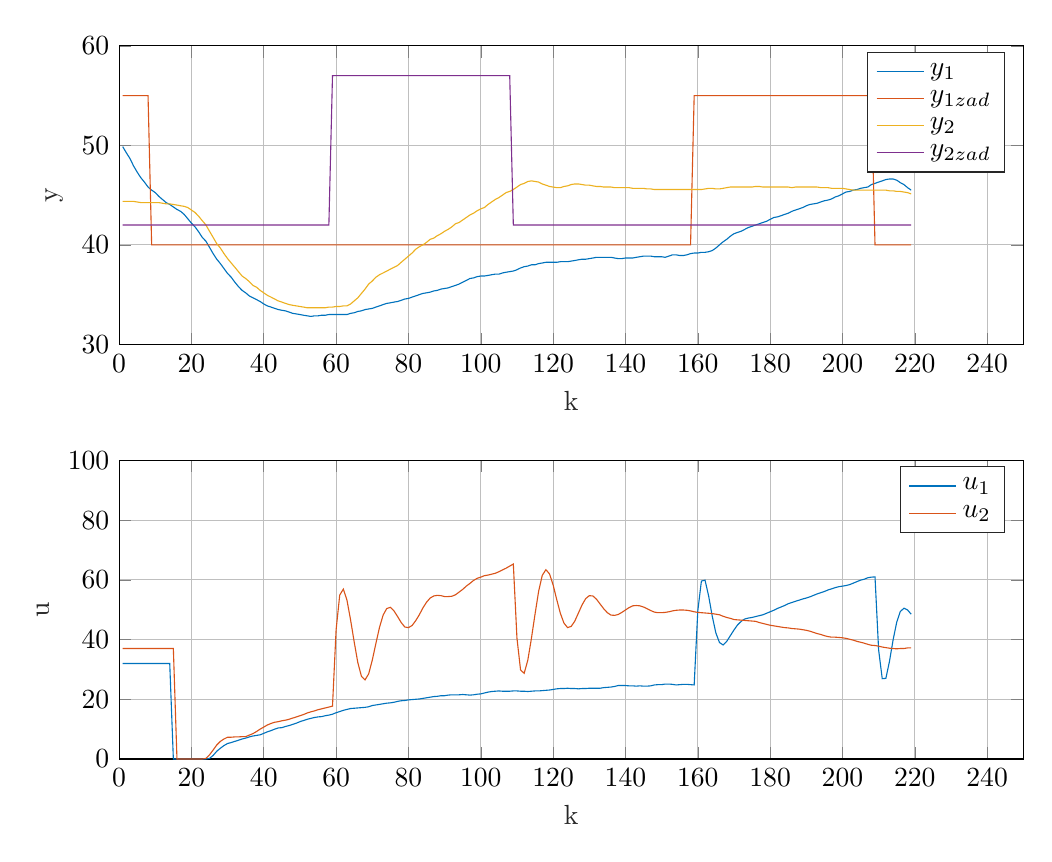
\begin{tikzpicture}

\begin{axis}[%
width=4.521in,
height=1.493in,
at={(0.758in,2.554in)},
scale only axis,
xmin=0,
xmax=250,
xlabel style={font=\color{white!15!black}},
xlabel={k},
ymin=30,
ymax=60,
ylabel style={font=\color{white!15!black}},
ylabel={y},
axis background/.style={fill=white},
xmajorgrids,
ymajorgrids,
legend style={legend cell align=left, align=left, draw=white!15!black}
]
\addplot [color=mycolor1]
  table[row sep=crcr]{%
1	49.87\\
2	49.25\\
3	48.68\\
4	47.93\\
5	47.31\\
6	46.75\\
7	46.31\\
8	45.81\\
9	45.5\\
10	45.25\\
11	44.87\\
12	44.56\\
13	44.25\\
14	44.06\\
15	43.81\\
16	43.56\\
17	43.37\\
18	43.06\\
19	42.62\\
20	42.18\\
21	41.81\\
22	41.31\\
23	40.75\\
24	40.37\\
25	39.75\\
26	39.12\\
27	38.56\\
28	38.12\\
29	37.62\\
30	37.12\\
31	36.75\\
32	36.25\\
33	35.81\\
34	35.43\\
35	35.18\\
36	34.87\\
37	34.68\\
38	34.5\\
39	34.31\\
40	34.06\\
41	33.87\\
42	33.75\\
43	33.62\\
44	33.5\\
45	33.43\\
46	33.37\\
47	33.25\\
48	33.12\\
49	33.06\\
50	33\\
51	32.93\\
52	32.87\\
53	32.81\\
54	32.87\\
55	32.87\\
56	32.93\\
57	32.93\\
58	33\\
59	33\\
60	33\\
61	33\\
62	33\\
63	33\\
64	33.12\\
65	33.18\\
66	33.31\\
67	33.37\\
68	33.5\\
69	33.56\\
70	33.62\\
71	33.75\\
72	33.87\\
73	34\\
74	34.12\\
75	34.18\\
76	34.25\\
77	34.31\\
78	34.43\\
79	34.56\\
80	34.62\\
81	34.75\\
82	34.87\\
83	35\\
84	35.12\\
85	35.18\\
86	35.25\\
87	35.37\\
88	35.43\\
89	35.56\\
90	35.62\\
91	35.68\\
92	35.81\\
93	35.93\\
94	36.06\\
95	36.25\\
96	36.43\\
97	36.62\\
98	36.68\\
99	36.81\\
100	36.87\\
101	36.87\\
102	36.93\\
103	37\\
104	37.06\\
105	37.06\\
106	37.18\\
107	37.25\\
108	37.31\\
109	37.37\\
110	37.5\\
111	37.68\\
112	37.81\\
113	37.87\\
114	38\\
115	38\\
116	38.12\\
117	38.18\\
118	38.25\\
119	38.25\\
120	38.25\\
121	38.25\\
122	38.31\\
123	38.31\\
124	38.31\\
125	38.37\\
126	38.43\\
127	38.5\\
128	38.56\\
129	38.56\\
130	38.62\\
131	38.68\\
132	38.75\\
133	38.75\\
134	38.75\\
135	38.75\\
136	38.75\\
137	38.68\\
138	38.62\\
139	38.62\\
140	38.68\\
141	38.68\\
142	38.68\\
143	38.75\\
144	38.81\\
145	38.87\\
146	38.87\\
147	38.87\\
148	38.81\\
149	38.81\\
150	38.81\\
151	38.75\\
152	38.87\\
153	39\\
154	39\\
155	38.93\\
156	38.93\\
157	39\\
158	39.12\\
159	39.18\\
160	39.18\\
161	39.25\\
162	39.25\\
163	39.31\\
164	39.43\\
165	39.68\\
166	40\\
167	40.31\\
168	40.56\\
169	40.87\\
170	41.12\\
171	41.25\\
172	41.37\\
173	41.56\\
174	41.75\\
175	41.87\\
176	42\\
177	42.12\\
178	42.25\\
179	42.37\\
180	42.56\\
181	42.75\\
182	42.81\\
183	42.93\\
184	43.06\\
185	43.18\\
186	43.37\\
187	43.5\\
188	43.62\\
189	43.75\\
190	43.93\\
191	44.06\\
192	44.12\\
193	44.18\\
194	44.31\\
195	44.43\\
196	44.5\\
197	44.62\\
198	44.81\\
199	44.93\\
200	45.12\\
201	45.31\\
202	45.37\\
203	45.5\\
204	45.56\\
205	45.68\\
206	45.75\\
207	45.81\\
208	46.06\\
209	46.18\\
210	46.31\\
211	46.43\\
212	46.56\\
213	46.62\\
214	46.62\\
215	46.5\\
216	46.25\\
217	46.06\\
218	45.75\\
219	45.5\\
};
\addlegendentry{$\text{y}_\text{1}$}

\addplot [color=mycolor2]
  table[row sep=crcr]{%
1	55\\
2	55\\
3	55\\
4	55\\
5	55\\
6	55\\
7	55\\
8	55\\
9	40\\
10	40\\
11	40\\
12	40\\
13	40\\
14	40\\
15	40\\
16	40\\
17	40\\
18	40\\
19	40\\
20	40\\
21	40\\
22	40\\
23	40\\
24	40\\
25	40\\
26	40\\
27	40\\
28	40\\
29	40\\
30	40\\
31	40\\
32	40\\
33	40\\
34	40\\
35	40\\
36	40\\
37	40\\
38	40\\
39	40\\
40	40\\
41	40\\
42	40\\
43	40\\
44	40\\
45	40\\
46	40\\
47	40\\
48	40\\
49	40\\
50	40\\
51	40\\
52	40\\
53	40\\
54	40\\
55	40\\
56	40\\
57	40\\
58	40\\
59	40\\
60	40\\
61	40\\
62	40\\
63	40\\
64	40\\
65	40\\
66	40\\
67	40\\
68	40\\
69	40\\
70	40\\
71	40\\
72	40\\
73	40\\
74	40\\
75	40\\
76	40\\
77	40\\
78	40\\
79	40\\
80	40\\
81	40\\
82	40\\
83	40\\
84	40\\
85	40\\
86	40\\
87	40\\
88	40\\
89	40\\
90	40\\
91	40\\
92	40\\
93	40\\
94	40\\
95	40\\
96	40\\
97	40\\
98	40\\
99	40\\
100	40\\
101	40\\
102	40\\
103	40\\
104	40\\
105	40\\
106	40\\
107	40\\
108	40\\
109	40\\
110	40\\
111	40\\
112	40\\
113	40\\
114	40\\
115	40\\
116	40\\
117	40\\
118	40\\
119	40\\
120	40\\
121	40\\
122	40\\
123	40\\
124	40\\
125	40\\
126	40\\
127	40\\
128	40\\
129	40\\
130	40\\
131	40\\
132	40\\
133	40\\
134	40\\
135	40\\
136	40\\
137	40\\
138	40\\
139	40\\
140	40\\
141	40\\
142	40\\
143	40\\
144	40\\
145	40\\
146	40\\
147	40\\
148	40\\
149	40\\
150	40\\
151	40\\
152	40\\
153	40\\
154	40\\
155	40\\
156	40\\
157	40\\
158	40\\
159	55\\
160	55\\
161	55\\
162	55\\
163	55\\
164	55\\
165	55\\
166	55\\
167	55\\
168	55\\
169	55\\
170	55\\
171	55\\
172	55\\
173	55\\
174	55\\
175	55\\
176	55\\
177	55\\
178	55\\
179	55\\
180	55\\
181	55\\
182	55\\
183	55\\
184	55\\
185	55\\
186	55\\
187	55\\
188	55\\
189	55\\
190	55\\
191	55\\
192	55\\
193	55\\
194	55\\
195	55\\
196	55\\
197	55\\
198	55\\
199	55\\
200	55\\
201	55\\
202	55\\
203	55\\
204	55\\
205	55\\
206	55\\
207	55\\
208	55\\
209	40\\
210	40\\
211	40\\
212	40\\
213	40\\
214	40\\
215	40\\
216	40\\
217	40\\
218	40\\
219	40\\
};
\addlegendentry{$\text{y}_{\text{1zad}}$}

\addplot [color=mycolor3]
  table[row sep=crcr]{%
1	44.37\\
2	44.37\\
3	44.37\\
4	44.37\\
5	44.31\\
6	44.25\\
7	44.25\\
8	44.25\\
9	44.25\\
10	44.25\\
11	44.25\\
12	44.18\\
13	44.12\\
14	44.12\\
15	44.06\\
16	44\\
17	43.93\\
18	43.87\\
19	43.75\\
20	43.5\\
21	43.25\\
22	42.87\\
23	42.43\\
24	42\\
25	41.37\\
26	40.75\\
27	40.12\\
28	39.68\\
29	39.12\\
30	38.62\\
31	38.18\\
32	37.75\\
33	37.31\\
34	36.87\\
35	36.62\\
36	36.31\\
37	35.93\\
38	35.75\\
39	35.43\\
40	35.18\\
41	34.93\\
42	34.75\\
43	34.56\\
44	34.37\\
45	34.25\\
46	34.12\\
47	34\\
48	33.93\\
49	33.87\\
50	33.81\\
51	33.75\\
52	33.68\\
53	33.68\\
54	33.68\\
55	33.68\\
56	33.68\\
57	33.68\\
58	33.75\\
59	33.75\\
60	33.81\\
61	33.81\\
62	33.87\\
63	33.87\\
64	34.06\\
65	34.37\\
66	34.68\\
67	35.12\\
68	35.56\\
69	36.06\\
70	36.37\\
71	36.75\\
72	37\\
73	37.18\\
74	37.37\\
75	37.56\\
76	37.75\\
77	37.93\\
78	38.25\\
79	38.56\\
80	38.87\\
81	39.18\\
82	39.56\\
83	39.81\\
84	40\\
85	40.25\\
86	40.56\\
87	40.68\\
88	40.93\\
89	41.12\\
90	41.37\\
91	41.56\\
92	41.81\\
93	42.12\\
94	42.25\\
95	42.5\\
96	42.75\\
97	43\\
98	43.18\\
99	43.43\\
100	43.62\\
101	43.75\\
102	44.06\\
103	44.31\\
104	44.56\\
105	44.75\\
106	45\\
107	45.25\\
108	45.37\\
109	45.56\\
110	45.81\\
111	46.06\\
112	46.18\\
113	46.37\\
114	46.43\\
115	46.37\\
116	46.31\\
117	46.12\\
118	46\\
119	45.87\\
120	45.81\\
121	45.75\\
122	45.75\\
123	45.87\\
124	45.93\\
125	46.06\\
126	46.12\\
127	46.12\\
128	46.06\\
129	46\\
130	46\\
131	45.93\\
132	45.87\\
133	45.87\\
134	45.81\\
135	45.81\\
136	45.81\\
137	45.75\\
138	45.75\\
139	45.75\\
140	45.75\\
141	45.75\\
142	45.68\\
143	45.68\\
144	45.68\\
145	45.68\\
146	45.62\\
147	45.62\\
148	45.56\\
149	45.56\\
150	45.56\\
151	45.56\\
152	45.56\\
153	45.56\\
154	45.56\\
155	45.56\\
156	45.56\\
157	45.56\\
158	45.56\\
159	45.56\\
160	45.56\\
161	45.56\\
162	45.62\\
163	45.68\\
164	45.68\\
165	45.62\\
166	45.62\\
167	45.68\\
168	45.75\\
169	45.81\\
170	45.81\\
171	45.81\\
172	45.81\\
173	45.81\\
174	45.81\\
175	45.81\\
176	45.87\\
177	45.87\\
178	45.81\\
179	45.81\\
180	45.81\\
181	45.81\\
182	45.81\\
183	45.81\\
184	45.81\\
185	45.81\\
186	45.75\\
187	45.81\\
188	45.81\\
189	45.81\\
190	45.81\\
191	45.81\\
192	45.81\\
193	45.81\\
194	45.75\\
195	45.75\\
196	45.75\\
197	45.68\\
198	45.68\\
199	45.68\\
200	45.68\\
201	45.62\\
202	45.56\\
203	45.5\\
204	45.5\\
205	45.5\\
206	45.5\\
207	45.5\\
208	45.5\\
209	45.5\\
210	45.5\\
211	45.5\\
212	45.5\\
213	45.43\\
214	45.43\\
215	45.37\\
216	45.37\\
217	45.31\\
218	45.25\\
219	45.12\\
};
\addlegendentry{$\text{y}_\text{2}$}

\addplot [color=mycolor4]
  table[row sep=crcr]{%
1	42\\
2	42\\
3	42\\
4	42\\
5	42\\
6	42\\
7	42\\
8	42\\
9	42\\
10	42\\
11	42\\
12	42\\
13	42\\
14	42\\
15	42\\
16	42\\
17	42\\
18	42\\
19	42\\
20	42\\
21	42\\
22	42\\
23	42\\
24	42\\
25	42\\
26	42\\
27	42\\
28	42\\
29	42\\
30	42\\
31	42\\
32	42\\
33	42\\
34	42\\
35	42\\
36	42\\
37	42\\
38	42\\
39	42\\
40	42\\
41	42\\
42	42\\
43	42\\
44	42\\
45	42\\
46	42\\
47	42\\
48	42\\
49	42\\
50	42\\
51	42\\
52	42\\
53	42\\
54	42\\
55	42\\
56	42\\
57	42\\
58	42\\
59	57\\
60	57\\
61	57\\
62	57\\
63	57\\
64	57\\
65	57\\
66	57\\
67	57\\
68	57\\
69	57\\
70	57\\
71	57\\
72	57\\
73	57\\
74	57\\
75	57\\
76	57\\
77	57\\
78	57\\
79	57\\
80	57\\
81	57\\
82	57\\
83	57\\
84	57\\
85	57\\
86	57\\
87	57\\
88	57\\
89	57\\
90	57\\
91	57\\
92	57\\
93	57\\
94	57\\
95	57\\
96	57\\
97	57\\
98	57\\
99	57\\
100	57\\
101	57\\
102	57\\
103	57\\
104	57\\
105	57\\
106	57\\
107	57\\
108	57\\
109	42\\
110	42\\
111	42\\
112	42\\
113	42\\
114	42\\
115	42\\
116	42\\
117	42\\
118	42\\
119	42\\
120	42\\
121	42\\
122	42\\
123	42\\
124	42\\
125	42\\
126	42\\
127	42\\
128	42\\
129	42\\
130	42\\
131	42\\
132	42\\
133	42\\
134	42\\
135	42\\
136	42\\
137	42\\
138	42\\
139	42\\
140	42\\
141	42\\
142	42\\
143	42\\
144	42\\
145	42\\
146	42\\
147	42\\
148	42\\
149	42\\
150	42\\
151	42\\
152	42\\
153	42\\
154	42\\
155	42\\
156	42\\
157	42\\
158	42\\
159	42\\
160	42\\
161	42\\
162	42\\
163	42\\
164	42\\
165	42\\
166	42\\
167	42\\
168	42\\
169	42\\
170	42\\
171	42\\
172	42\\
173	42\\
174	42\\
175	42\\
176	42\\
177	42\\
178	42\\
179	42\\
180	42\\
181	42\\
182	42\\
183	42\\
184	42\\
185	42\\
186	42\\
187	42\\
188	42\\
189	42\\
190	42\\
191	42\\
192	42\\
193	42\\
194	42\\
195	42\\
196	42\\
197	42\\
198	42\\
199	42\\
200	42\\
201	42\\
202	42\\
203	42\\
204	42\\
205	42\\
206	42\\
207	42\\
208	42\\
209	42\\
210	42\\
211	42\\
212	42\\
213	42\\
214	42\\
215	42\\
216	42\\
217	42\\
218	42\\
219	42\\
};
\addlegendentry{$\text{y}_{\text{2zad}}$}

\end{axis}

\begin{axis}[%
width=4.521in,
height=1.493in,
at={(0.758in,0.481in)},
scale only axis,
xmin=0,
xmax=250,
xlabel style={font=\color{white!15!black}},
xlabel={k},
ymin=0,
ymax=100,
ylabel style={font=\color{white!15!black}},
ylabel={u},
axis background/.style={fill=white},
xmajorgrids,
ymajorgrids,
legend style={legend cell align=left, align=left, draw=white!15!black}
]
\addplot [color=mycolor1]
  table[row sep=crcr]{%
1	32\\
2	32\\
3	32\\
4	32\\
5	32\\
6	32\\
7	32\\
8	32\\
9	32\\
10	32\\
11	32\\
12	32\\
13	32\\
14	32\\
15	0\\
16	0\\
17	0\\
18	0\\
19	0\\
20	0\\
21	0\\
22	0\\
23	0\\
24	0\\
25	0.2\\
26	1.2\\
27	2.6\\
28	3.6\\
29	4.5\\
30	5.2\\
31	5.5\\
32	5.9\\
33	6.3\\
34	6.7\\
35	7\\
36	7.4\\
37	7.7\\
38	7.9\\
39	8.1\\
40	8.6\\
41	9.1\\
42	9.5\\
43	10\\
44	10.4\\
45	10.5\\
46	10.9\\
47	11.2\\
48	11.6\\
49	12\\
50	12.5\\
51	12.9\\
52	13.3\\
53	13.6\\
54	13.9\\
55	14.1\\
56	14.2\\
57	14.5\\
58	14.7\\
59	15\\
60	15.5\\
61	15.9\\
62	16.3\\
63	16.6\\
64	16.9\\
65	17\\
66	17.1\\
67	17.2\\
68	17.3\\
69	17.5\\
70	17.9\\
71	18.1\\
72	18.3\\
73	18.5\\
74	18.7\\
75	18.8\\
76	19\\
77	19.3\\
78	19.5\\
79	19.6\\
80	19.8\\
81	19.9\\
82	20\\
83	20.1\\
84	20.3\\
85	20.5\\
86	20.7\\
87	20.9\\
88	21\\
89	21.2\\
90	21.2\\
91	21.4\\
92	21.5\\
93	21.5\\
94	21.5\\
95	21.6\\
96	21.5\\
97	21.4\\
98	21.5\\
99	21.7\\
100	21.8\\
101	22.1\\
102	22.4\\
103	22.6\\
104	22.7\\
105	22.8\\
106	22.7\\
107	22.7\\
108	22.7\\
109	22.8\\
110	22.8\\
111	22.7\\
112	22.7\\
113	22.6\\
114	22.7\\
115	22.8\\
116	22.8\\
117	22.9\\
118	23\\
119	23.1\\
120	23.3\\
121	23.5\\
122	23.6\\
123	23.6\\
124	23.7\\
125	23.6\\
126	23.6\\
127	23.5\\
128	23.6\\
129	23.6\\
130	23.7\\
131	23.7\\
132	23.7\\
133	23.7\\
134	23.9\\
135	24\\
136	24.1\\
137	24.3\\
138	24.6\\
139	24.6\\
140	24.6\\
141	24.5\\
142	24.5\\
143	24.4\\
144	24.5\\
145	24.4\\
146	24.4\\
147	24.5\\
148	24.8\\
149	24.9\\
150	24.9\\
151	25.1\\
152	25.1\\
153	25\\
154	24.8\\
155	24.9\\
156	25\\
157	25\\
158	24.9\\
159	24.8\\
160	49.6\\
161	59.6\\
162	59.9\\
163	54.6\\
164	47.8\\
165	42.2\\
166	39\\
167	38.2\\
168	39.4\\
169	41.3\\
170	43.2\\
171	44.9\\
172	46.1\\
173	46.9\\
174	47.2\\
175	47.4\\
176	47.7\\
177	48\\
178	48.3\\
179	48.8\\
180	49.3\\
181	49.8\\
182	50.4\\
183	50.9\\
184	51.4\\
185	52\\
186	52.4\\
187	52.8\\
188	53.2\\
189	53.6\\
190	53.9\\
191	54.3\\
192	54.8\\
193	55.3\\
194	55.7\\
195	56.1\\
196	56.6\\
197	57\\
198	57.4\\
199	57.7\\
200	57.9\\
201	58.1\\
202	58.4\\
203	58.9\\
204	59.4\\
205	59.9\\
206	60.2\\
207	60.7\\
208	60.9\\
209	61\\
210	36.5\\
211	26.9\\
212	27\\
213	32.7\\
214	39.9\\
215	45.8\\
216	49.4\\
217	50.5\\
218	49.9\\
219	48.5\\
};
\addlegendentry{$\text{u}_\text{1}$}

\addplot [color=mycolor2]
  table[row sep=crcr]{%
1	37\\
2	37\\
3	37\\
4	37\\
5	37\\
6	37\\
7	37\\
8	37\\
9	37\\
10	37\\
11	37\\
12	37\\
13	37\\
14	37\\
15	37\\
16	0\\
17	0\\
18	0\\
19	0\\
20	0\\
21	0\\
22	0\\
23	0\\
24	0.2\\
25	1.4\\
26	3\\
27	4.7\\
28	5.9\\
29	6.7\\
30	7.3\\
31	7.3\\
32	7.4\\
33	7.4\\
34	7.5\\
35	7.5\\
36	8\\
37	8.5\\
38	9.2\\
39	10\\
40	10.7\\
41	11.4\\
42	11.9\\
43	12.3\\
44	12.5\\
45	12.8\\
46	13\\
47	13.3\\
48	13.7\\
49	14.1\\
50	14.5\\
51	14.9\\
52	15.4\\
53	15.8\\
54	16.1\\
55	16.5\\
56	16.8\\
57	17.1\\
58	17.4\\
59	17.7\\
60	43.3\\
61	54.9\\
62	56.9\\
63	53.2\\
64	46.6\\
65	39.2\\
66	32.3\\
67	27.7\\
68	26.5\\
69	28.5\\
70	33.1\\
71	38.7\\
72	44.1\\
73	48.2\\
74	50.4\\
75	50.8\\
76	49.6\\
77	47.7\\
78	45.7\\
79	44.2\\
80	44\\
81	44.7\\
82	46.3\\
83	48.3\\
84	50.6\\
85	52.5\\
86	53.9\\
87	54.6\\
88	54.8\\
89	54.7\\
90	54.4\\
91	54.4\\
92	54.5\\
93	55\\
94	55.9\\
95	56.8\\
96	57.9\\
97	58.8\\
98	59.8\\
99	60.5\\
100	60.9\\
101	61.4\\
102	61.6\\
103	61.9\\
104	62.2\\
105	62.7\\
106	63.3\\
107	63.9\\
108	64.6\\
109	65.3\\
110	40.5\\
111	29.8\\
112	28.7\\
113	33.1\\
114	40.4\\
115	48.5\\
116	56.2\\
117	61.5\\
118	63.4\\
119	62\\
120	58.3\\
121	53.4\\
122	48.8\\
123	45.5\\
124	44\\
125	44.4\\
126	46.2\\
127	48.9\\
128	51.6\\
129	53.7\\
130	54.7\\
131	54.6\\
132	53.5\\
133	51.9\\
134	50.3\\
135	49\\
136	48.2\\
137	48.1\\
138	48.4\\
139	49.1\\
140	49.9\\
141	50.7\\
142	51.3\\
143	51.4\\
144	51.3\\
145	50.9\\
146	50.3\\
147	49.7\\
148	49.2\\
149	49\\
150	49\\
151	49.1\\
152	49.3\\
153	49.6\\
154	49.8\\
155	49.9\\
156	49.9\\
157	49.8\\
158	49.6\\
159	49.3\\
160	49.1\\
161	49\\
162	48.9\\
163	48.8\\
164	48.7\\
165	48.5\\
166	48.3\\
167	47.8\\
168	47.4\\
169	47.1\\
170	46.7\\
171	46.6\\
172	46.5\\
173	46.4\\
174	46.3\\
175	46.2\\
176	46.1\\
177	45.7\\
178	45.4\\
179	45.1\\
180	44.8\\
181	44.6\\
182	44.4\\
183	44.2\\
184	44\\
185	43.9\\
186	43.7\\
187	43.6\\
188	43.5\\
189	43.3\\
190	43.1\\
191	42.8\\
192	42.4\\
193	42\\
194	41.7\\
195	41.3\\
196	41\\
197	40.8\\
198	40.8\\
199	40.7\\
200	40.6\\
201	40.4\\
202	40.1\\
203	39.8\\
204	39.4\\
205	39.1\\
206	38.8\\
207	38.4\\
208	38.1\\
209	38\\
210	37.8\\
211	37.5\\
212	37.3\\
213	37.1\\
214	37\\
215	36.9\\
216	37\\
217	37\\
218	37.2\\
219	37.2\\
};
\addlegendentry{$\text{u}_{\text{2}}$}

\end{axis}
\end{tikzpicture}%
    \caption{Eksperyment z regulatorem DMC}
    \label{lab:zad4:figure:wektorS2}
 \end{figure}
\fi

\newpage
